\documentclass[Ex4_Zusammenfassung.tex]{subfiles}

\begin{document}

\chapter{ Ex \rom{4} -- Atomphysik}

 Wer den Ursprung des einleitend falsch zugeordneten Zitats kennt, der wird sofort assoziieren, dass wir in dieser Vorlesung versuchen zu erkennen, was die Welt im Innersten zusammenhält. Wir wollen in der Kern-- und Teilchenphysik die Struktur der Materie auf kleinster Skala beschreiben. Unsere Form von Magie nennt sich dabei Mathematik, wir werden jedoch versuchen nur an seltenen Stellen ihre Sätze ungeprüft zu gebrauchen um so einen Pakt mit Mephisto zu vermeiden. Wie schon in der Ex \rom{3} werden wir feststellen, dass manche Modelle auf kleinster Ebene nicht mehr zutreffen und neue Formalismen und Betrachtungsweisen unumgänglich sind. In dieser Vorlesung fällt buchstäblich vieles vom Himmel, aber solange man es schafft, den Überblick zu behalten, verliert man trotzdem nicht die Freude an der Thematik.\\

Jetzt aber zum Inhalt: wir setzen die Grundlagen der Quantenmechanik (z.B. aus Ex \rom{3}) voraus und betrachten zunächst noch einmal die Elektronenhüllen von Atomen. Richtig los geht es mit Stoßprozessen von Teilchen, wie wir sie nur mithilfe großer Beschleuniger erzeugen und auswerten können. Wir werden dann in Detektoren eine Winkelverteilung der Stoßprodukte beobachten und Größen wie Energie und Ladung ermitteln, um Rückschlüsse auf die Wechselwirkungen während des Stoßprozesses zu ziehen. Wegen der Unschärfe sind die Prozesse eine Art ''Black Box'' Problem, welches wir mit Feynman--Diagrammen darzustellen versuchen. 

\subsection*{Notation und Werte für Konstanten (laut Vorlesung)}
\begin{align*}
	e^2 &= \frac{q_e^2}{4\pi \epsilon_{0}} = \SI{1.44}{MeV fm}  \\
	\SI{1}{eV} &= \SI{1.6E-19}{J}  \\
	\SI{1}{fm} &= \SI{1E-15}{m}\\ 
	\SI{1}{u} &=  \SI{932}{MeV/c^2} = \SI{1.66E-27}{kg} \\
	\hslash &= \SI{6.58E-16}{eV s}= \SI{1.05E-34}{Js} \\
	\alpha &= \frac {e^2}{c \hslash} = \frac{1}{137} \\
	c &= \SI{3E8}{m/s}
\end{align*} 

\section{Spektroskopische Notation}
Um den (stationären) Zustand einer Unterschale nl anzugeben, führen wir die spektroskopische Notation ein: 
\begin{equation}
\centering \boxed{ n \ ^{2S+1}L_J }
\end{equation}
wobei die Drehimpulse und der Spin
\begin{align}
	\vec L &:= \sum_{i} \vec{\ell}_i \\
	\vec S &:= \sum_{i} \vec{s}_i \\
	\vec J &:= \sum_{i} \vec{s}_i + \vec{\ell}_i \stackrel{\text{jj}}{=} \sum_i \vec{j}_i \stackrel{\text{L--S}}{=} \vec{L} + \vec{S} \label{gesamtdrehimpuls}
\end{align}
vektoriell addiert werden, sodass die zu den Eigenwerten gehörenden Quantenzahlen $L,\ S,\ J$ für $L$ ganzzahlig und für $S,\ J$ auch halbzahlig sein können. Die verschiedenen $S,\ J$ müssen auch bei halbzahligen Werten Abstände von $1$ haben. In \ref{gesamtdrehimpuls} bedeuten die Anmerkungen jj und L--S, dass es sich um die jeweiligen Drehimpulskopplungen handelt. Darauf wird später eingegangen.\\

Die Notation für die Elemente des Periodensystems lautet
\begin{equation}
	\resizebox{0.6\hsize}{!}{%
	$\centering \boxed{^{\qquad Massenzahl \  \frac{m}{u} } _{Kernladungszahl \  Z} \  El ^{\ \frac{q}{q_e} \  Ionisierung}} $
	}
\end{equation}
\section{Hund'sche Regeln und Auswahlregeln}
Die Elektronen werden für die Grundzustände so aufgefüllt, dass die Bindungsenergie (negativ) minimiert wird, das heißt deren Betrag maximal wird. Zwischen den Unterschalen gilt folgende Reihenfolge: 
\begin{figure}[H]
	\centering
	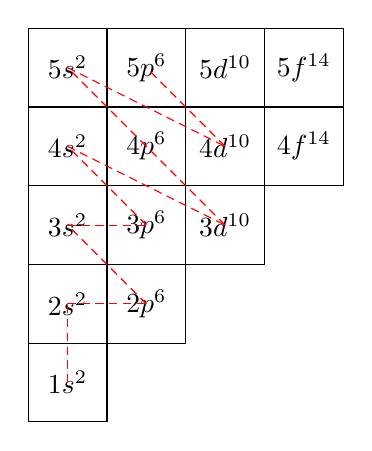
\begin{tikzpicture}
	\draw (0,0) +(-.5,-.5) rectangle ++(.5,.5);
	\draw (0,0) node{$1s^2$};
	\draw (0,1) +(-.5,-.5) rectangle ++(.5,.5);
	\draw (0,1) node{$2s^2$};
	\draw (0,2) +(-.5,-.5) rectangle ++(.5,.5);
	\draw (0,2) node{$3s^2$};
	\draw (0,3) +(-.5,-.5) rectangle ++(.5,.5);
	\draw (0,3) node{$4s^2$};
	\draw (0,4) +(-.5,-.5) rectangle ++(.5,.5);
	\draw (0,4) node{$5s^2$};

	\draw (1,1) +(-.5,-.5) rectangle ++(.5,.5);
	\draw (1,1) node{$2p^6$};
	\draw (1,2) +(-.5,-.5) rectangle ++(.5,.5);
	\draw (1,2) node{$3p^6$};
	\draw (1,3) +(-.5,-.5) rectangle ++(.5,.5);
	\draw (1,3) node{$4p^6$};
	\draw (1,4) +(-.5,-.5) rectangle ++(.5,.5);
	\draw (1,4) node{$5p^6$};

	\draw (2,2) +(-.5,-.5) rectangle ++(.5,.5);
	\draw (2,2) node{$3d^{10}$};
	\draw (2,3) +(-.5,-.5) rectangle ++(.5,.5);
	\draw (2,3) node{$4d^{10}$};
	\draw (2,4) +(-.5,-.5) rectangle ++(.5,.5);
	\draw (2,4) node{$5d^{10}$};

	\draw (3,3) +(-.5,-.5) rectangle ++(.5,.5);
	\draw (3,3) node{$4f^{14}$};
	\draw (3,4) +(-.5,-.5) rectangle ++(.5,.5);
	\draw (3,4) node{$5f^{14}$};

	\draw [draw = red, densely dashed] (0,0) -- (0,1);
	\draw [draw = red, densely dashed] (0,1) -- (1,1);
	\draw [draw = red, densely dashed] (1,1) -- (0,2);
	\draw [draw = red, densely dashed] (0,2) -- (1,2);
	\draw [draw = red, densely dashed] (1,2) -- (0,3);
	\draw [draw = red, densely dashed] (0,3) -- (2,2);
	\draw [draw = red, densely dashed] (2,2) -- (1,3);
	\draw [draw = red, densely dashed] (1,3) -- (0,4);
	\draw [draw = red, densely dashed] (0,4) -- (2,3);
	\draw [draw = red, densely dashed] (2,3) -- (1,4);
	\end{tikzpicture}
	\caption{Auffüllung der Grundzustände}
\end{figure}
	Pro Unterzustand hat man $ N_e = 2(2l+1) $ Elektronen. 
	Die Gesamtzahl der Elektronen in der n-ten Schale entspricht somit $ N_e = 2 \sum_{l}^{n-1} 2l+1 =   2n^2 $

Innerhalb einer Unterschale gelten für die Grundzustände die hierarchischen Hund'schen Regeln:
\colbox{\textbf{Hund'sche Regeln}}{ 
	\begin{enumerate}
		\item Der Gesamtspin wird maximal. Das heißt hier in diesem spezifischen Fall ist S gegeben durch $S = |\sum_i m_{s,i}| \stackrel{!}{=}$ max. 
		\item Der Gesamtdrehimpuls  wird maximal. Das heißt hier in diesem spezifischen Fall ist L gegeben durch  $L = |\sum_i m_{l,i}| \stackrel{!}{=}$ max.
		\item Ist die Unterschale bis zu (einschließlich) halb voll, so wird J minimal. Das heißt hier ist  $ J := \lvert M_L + M_S \rvert \stackrel{!}{=} \lvert L-S \rvert $ , bei mehr als halb vollen Unterschalen muss $ J \stackrel{!}{=} L+S $ sein. 
	\end{enumerate} 
}

Diese Regeln bestimmen die Feinstruktur des Elements. Regt man das Element an, so gelten diese Regeln nicht mehr. Möchte man im sogenannten Termschema verschiedene Zustände ihrer Energie nach ordnen (Energieniveaus), so ermittelt man den Grundzustand und verletzt dann die Regeln von unten nach oben.
Die  Schalen-/Orbitalübergänge werden von den sog. \textbf{Auswahlregeln} beherrscht, die wohlgemerkt nicht hierarchisch sind.
\colbox{\textbf{Auswahlregeln}}{
	\begin{enumerate}
		\item $ \Delta L \  \in $ \{-1,1\}  bei L-S-Kopplung
		\item $ \Delta M_L \   \in  $ \{-1,0,1\}  
		\item $ \Delta S =0 $ für leichte Atome $(Z <40)$
		\item $\Delta J \  \in $  \{-1,0,1\}   wobei $ \ J =0 \  \rightarrow J=0 \  \textbf{verboten} $
	\end{enumerate}
}

\section{Vielelektronenprobleme} 
Für Elemente mit mehr als einem Elektron gibt es keine analytische Lösung der Schrödinger-Gleichung, auch numerische Verfahren sind mit zunehmender Elektronenzahl extrem aufwändig. Wir machen deshalb folgende Näherungen:
\textbf{Alkaliatome} (1.Hauptgruppe)
\begin{itemize}
\item Alkaliatome haben nur ein Elektron außerhalb geschlossener Schalen. Die Grundzustände sind immer $ \ ^{2}S_{\frac{1}{2}} $ ( $ n  \in \{2,3,4,...\} $ nicht notiert).
\item Wir betrachten zu Näherung ein \textbf{effektives Potential} $ V_{eff}(r) $ \newline \newline
 $ V_{eff}(r) = - \frac{e^2 Z_{eff}(r)}{r} $ mit $ 1 < Z_{eff}(r) < Z $ \  und  $ Z_ {eff} \stackrel{r\rightarrow \infty}{\rightarrow} 1, \ Z_{eff} \stackrel{r \rightarrow 0}{\rightarrow} Z $
 
\begin{figure}[h]
\centering
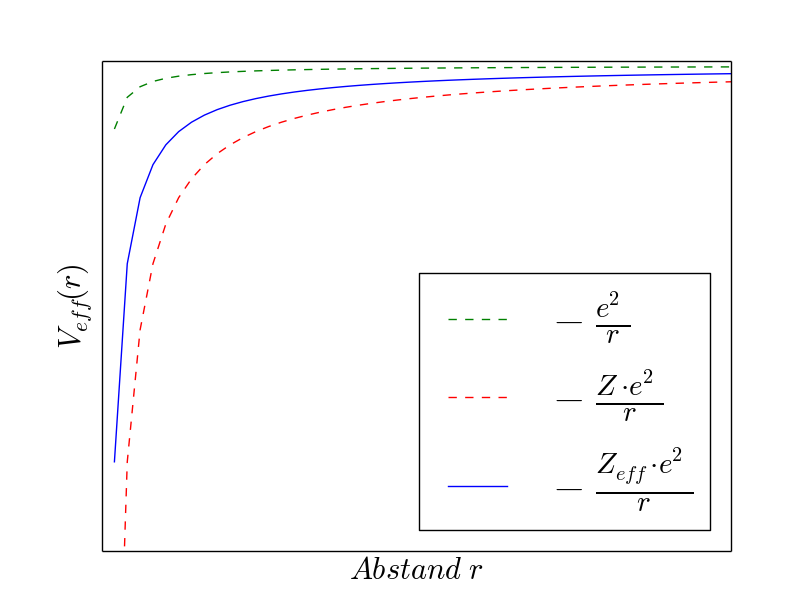
\includegraphics[height= 6cm, width=9cm]{effpot.png}
\caption{ Effektives Potential }
\end{figure}
 \item Dies hebt die $ E_n $ --Entartung bezüglich Z bereits auf (Feinstruktur): \newline
$ E_n(s) < E_n(p) < E_n(d) < E_n(f)$ (für kleine n am stärksten)
\item Für große n und r (wasserstoffähnlich) lässt sich dies so schreiben: 
	 \begin{equation}
 	E_{n,l} = -E_0 \frac{Z_{eff}^2}{n^2} = - \frac{E_0}{n_{eff}^2} = - \frac{E_0}{(n-\delta_{n,l})^2} \qquad E_0 = \SI{13.6}{eV}
 	\end{equation}
	wobei $\delta_{n,l} $ der sog. \textbf{Quantendefekt} ist: $ \delta_{n,l} = n - \sqrt{\frac{E_0}{-E_{n,l}}} \newline  E_{n,l} <  0  $ ist die real gemessene Energie. 

\end{itemize}
Um allgemeine Vielelektronenprobleme zu lösen, können wir (zumindest bis jetzt) nur nähern indem wir zur Lösung eines Elektrons die anderen Elektronen unabhängig voneinander gelöst haben und das entstehende $ V_{eff}(r) $ als \textbf{kugelsymmetrisch} angenommen wird.

Wir suchen deshalb eine  \textbf{Gesamtwellenfunktion} für N Teilchen.

Diese muss antisymmetrisch unter Vertauschung sein, wir nehmen zusätzlich an, dass sie sich als Produkt der Einteilchenwellenfunktionen schreiben lässt.

Analog zu $ \psi_{ges}(1,2) = \psi_1(1) \psi_2(2) - \psi_2(1) \psi_1(2) $  definieren wir die \\ \textbf{Slaterdeterminante}: 
	\begin{equation}
	  \psi_{ges}(r_1,...,r_N) \ = \  \frac{1}{\sqrt{N!}} \  det \begin{pmatrix} \psi_1(1) & \psi_1(2) & \dots & \psi_1(N) \\ \vdots & \vdots & \vdots & \vdots \\  \psi_N(1) & \psi_N(2) & \dots & \psi_N(N)  \end{pmatrix} 
	\end{equation}
Diese ist total antisymmetrisch unter Spaltenvertauschung und eine Summe aus $N!$ Produkten. 
\section{Moseley'sches-Gesetz}
Für Eletronen--Übergänge zwischen Zuständen wurde empirisch festgestellt, dass $ \sqrt{f} \propto Z $ ist, wobei $f$ die Frequenz des emittierten Lichts und $Z$ die Ladungszahl  ist. 

\begin{align}
	f &= \frac{E_0 (Z-b)^2}{h (1+\nicefrac{m_e}{M_{core}})} \left(\frac{1}{n_2^2} - \frac{1}{n_1^2}\right) \\ 
	\lambda \ & = \frac{ch(1+\nicefrac{m_e}{M_{core}})}{E_0 (Z-b)^2} \frac{1}{\nicefrac{1}{n_2^2} - \nicefrac{1}{n_1^2}} 
\end{align}
für Übergänge $ n_1 \rightarrow n_2 $, wobei $b$ die Abschirmkonstante ist.\\

Für das Wasserstoffatom entspricht das Moseley-Gesetz der Rydberg-Formel.

Für wasserstoffähnliche Atome gilt b=(Z-1) : \newline \quad K-Linien: $ n_2 = 1, \  K_{\alpha} :  n_1 = 2, \  K_{\beta}: n_1 = 3 $ \\ \newline
Für schwere Atome ($ Z > 40 $  )  gibt es zusätzlich: \newline \qquad L-Linien: $ n_2 = 2 , b \approx 7.4 , \ L_{\alpha} : \ n_1= 3 , \  L_{\beta}: n_1 = 4 $\\

Die Auswahlregeln müssen gelten.
\end{document}